% !TeX root = thesis.tex
\documentclass{master_thesis}
\addbibresource{refs.bib}

\begin{document}

\section{Results} \label{chap:results}

% The nucleus of your dissertation, the results chapter thoroughly explores your findings. This is where you present your data or original analysis, along with any visual aids, such as graphs or charts.

% For empirical dissertations, structure the results section by individual data findings, analyzed in depth one by one. For nonempirical dissertations, structure this section by themes, patterns, or trends you’ve noticed in your research.

% Don’t forget to relate your findings back to the central research question or thesis statement.

\subsection{Results from Manual Audit and Automated Tests}

\info{RQ2: What kind of errors can be caught by running automated accessibility tests on a component library?}

A summarized table was created from all violations and passes in automated tests and issues found in the manual audit. In this table, the results have been reduced to counts that can be analyzed using statistical methods (Appendix \ref{appendix:results-table}).

% summary of violations
The results show that addon-a11y did not report any violations for 27 (51\%) components out of 53 components after verifying the validity of these issues the number goes up to 31 (58\%) (Figure \ref{fig:audit-failed}). On average the automated testing tool found 1 violation per component. The maximum number of violations reported for a single component was 7 and the maximum number of valid violations was 6.

% summary of passes
4 components out of 53 did not have any passed checks and 22 did not have any valid passed checks (see figure \ref{fig:audit-passed}). This means that the number of components with no valid passed checks changed from 4\%  to 42\% after manually validating the results. The highest number of passes was 18 and that many issues were detected for \textit{Form} and \textit{Table} components. After validating the number of passes changed to 9 for \textit{Table} and 7 for \textit{Form}. The average number of passes for each component was 5 before and 2 after validating the results.

\begin{figure}[ht]
	\begin{subfigure}{0.45\textwidth}
	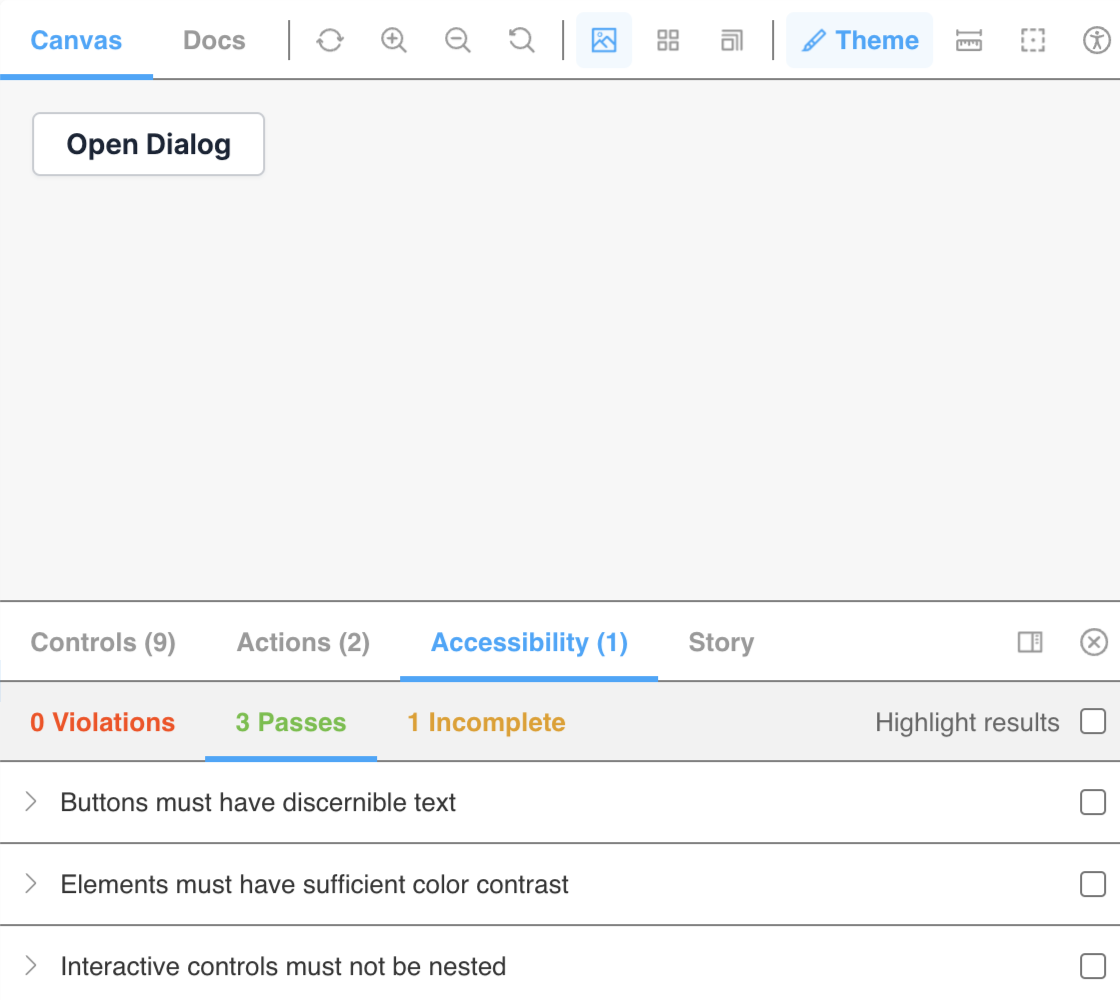
\includegraphics[width=\textwidth]{img/sb-button-trigger.png}
	\caption{Inital view of example. This is tested by addon-a11y.}
	\label{fig:sb-button-trigger-1}
	\end{subfigure}
	\hspace{0.05\textwidth}
	\begin{subfigure}{0.45\textwidth}
	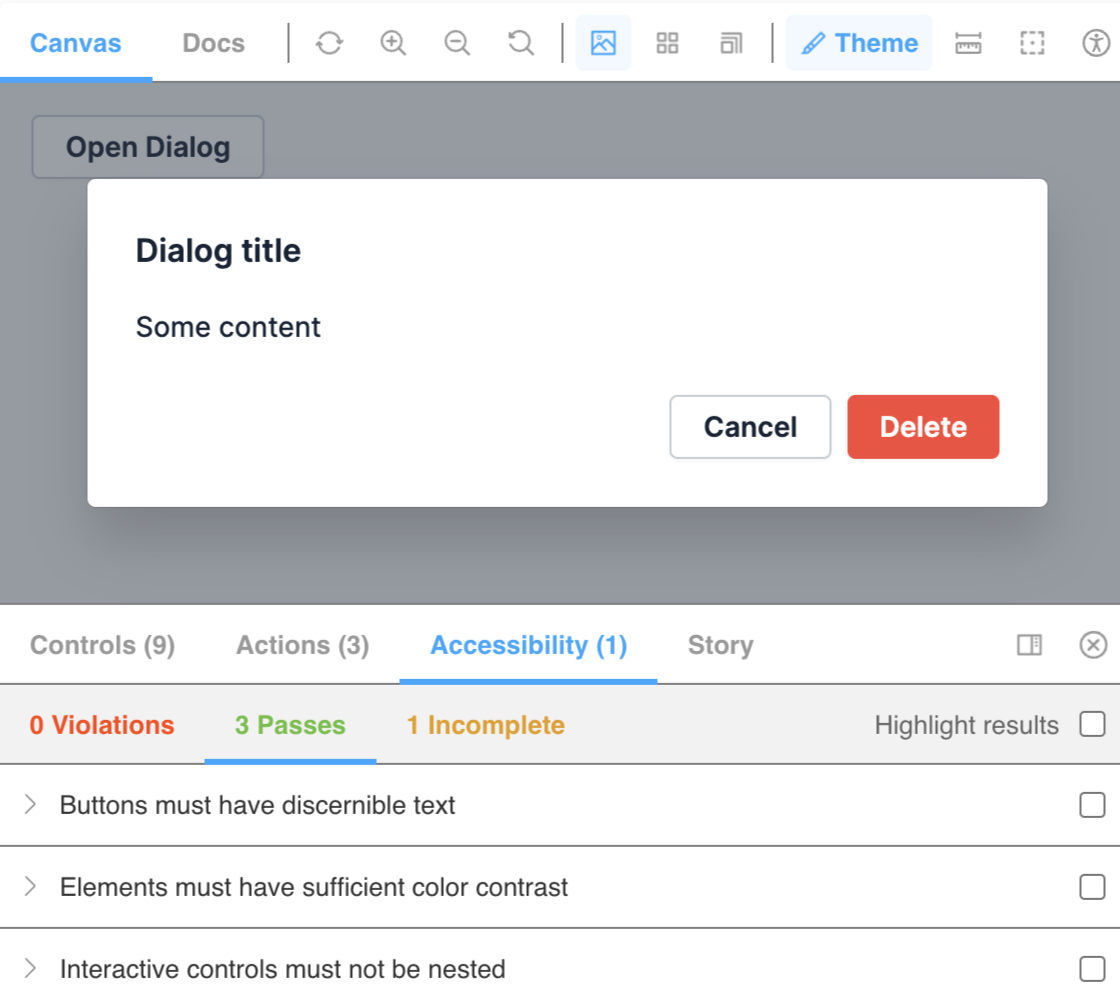
\includegraphics[width=\textwidth]{img/sb-button-trigger-open.png}
	\caption{Example after clicking the button and revealing the actual component.}
	\label{fig:sb-button-trigger-2}
	\end{subfigure}
\caption{Storybook example for Dialog component using button trigger}
\label{fig:sb-button-trigger}
\end{figure}

\begin{figure}[H]
	\begin{subfigure}{0.45\textwidth}
	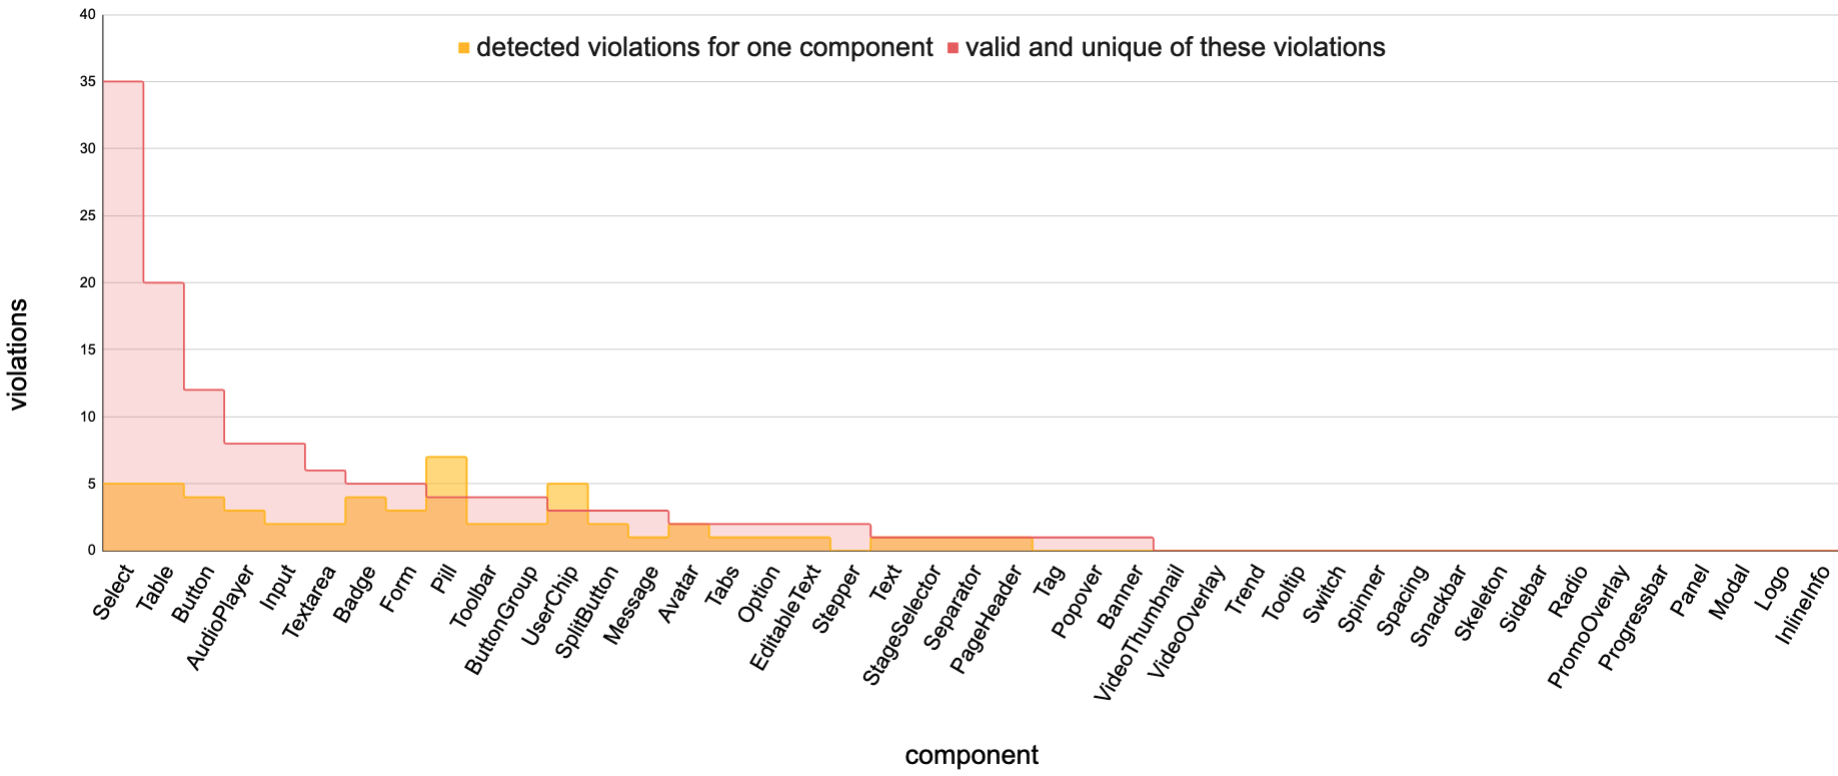
\includegraphics[height=0.9\textheight]{img/audit-failed.png}
	\caption{All violations reported by addon-a11y and how many of them are valid.}
	\label{fig:audit-failed}
	\end{subfigure}
	\hspace{0.05\textwidth}
	\begin{subfigure}{0.45\textwidth}
	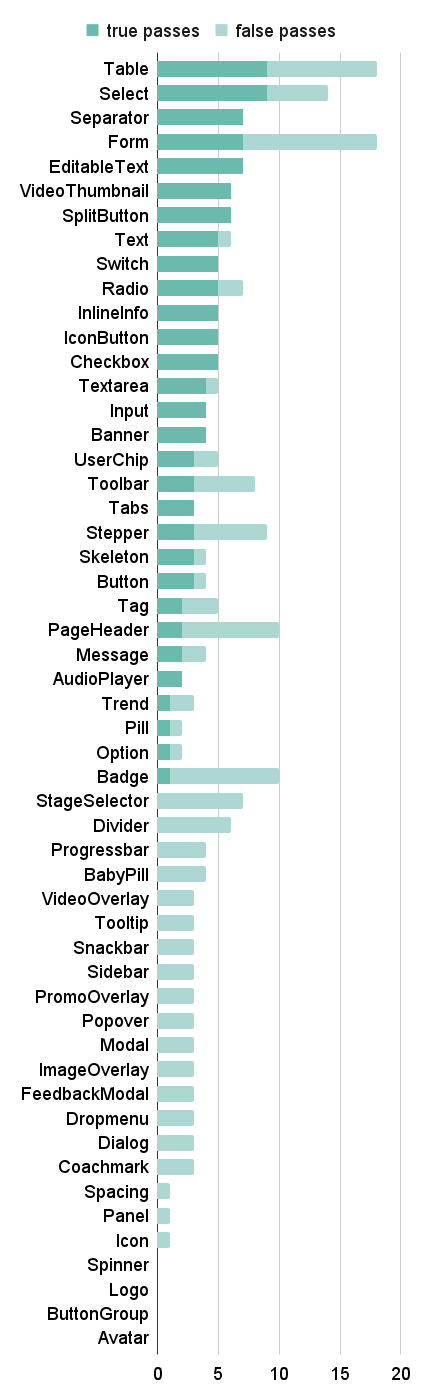
\includegraphics[height=0.9\textheight]{img/audit-passed.png}
	\caption{All passed checks reported by addon-a11y and how many of them are valid.}
	\label{fig:audit-passed}
	\end{subfigure}
\caption{All issues checked by addon-a11y}
\label{fig:audit-passed-failed}
\end{figure}

% summary of violations + passes
Looking at all the fails and passes gave a good overview of how many tests were run for each component. Out of 53 components that were tested, only 2 (4\%) did not get checked by addon-a11y at all, but some of these included false violations or passes. After validating the results the number of components not tested is 20 (38\%). This included components that become visible only when triggered by another element, like modals and popups that were displayed with a button as a trigger in the Storybook examples (Figure \ref{fig:sb-button-trigger}). In total, there were 11 components with examples like that and they can be seen in Figure \ref{fig:audit-passed} starting from \textit{VideoOverlay} and ending with \textit{Coachmark}.

The components that are displayed with a button trigger would normally open when triggered by something and the examples are intended to look similar to how they would be used in real life. Brick-ui, the simple playground that was set up for testing solutions in Storybook was used to explore different ways of mitigating this. Testing revealed that these kinds of examples could be improved in Storybook 7 by adding a user interaction that opens the component because accessibility tests are run after this interaction has been executed. In Storybook 6 the same thing could be achieved by opening the example manually and triggering a rerun of the accessibility checks. It is important to make sure that the opened component is rendered inside the div element with id="root" (or "storybook-root" in version 7). All 11 components were retested and accessibility checks could be triggered on one of the examples of \textit{Tooltip} and \textit{Modal}. It is possible to render all the components except \textit{VideoOverlay} and \textit{FeedbackModal} inside the root element. This means that with improved examples tests could be run for these components. At the time of the case study, there was a bug in axe-core that caused most of the components to be ignored even if all the requirements described above are fulfilled.

The remainder of the components that did not get tested by the addon included very simple components for spacing and visuals. These need further testing when they are being used in context to make sure that the visual info they are conveying is also included in text form. The results from manual testing did not reveal any further issues for 6 of these components. The components that have a trigger button in the example had the most additional issues. This is expected as due to the limitation of the examples the correct component was not evaluated by the tool.

Analyzing the validity of checks performed by addon-a11y further shows that from all passes and fails together a bit more than half are valid while 68\% of detected violations are correct and 51\% of passed checks were confirmed to be relevant (Figure \ref{fig:checks-validity}).

\begin{figure}[ht]
	\centering
	\begin{subfigure}{0.3\textwidth}
	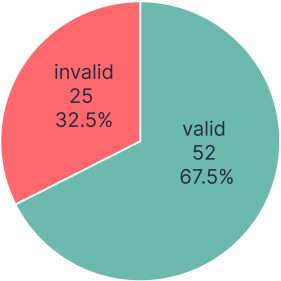
\includegraphics[width=\textwidth]{img/violations.png}
	\caption{How many of the detected violations are valid?}
	\label{fig:checks-validity-failed}
	\end{subfigure}
	\hspace{0.03\textwidth}
	\begin{subfigure}{0.3\textwidth}
	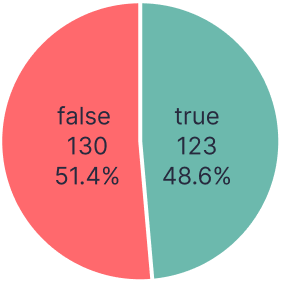
\includegraphics[width=\textwidth]{img/passes.png}
	\caption{How many of the passes are valid?}
	\label{fig:checks-validity-passed}
	\end{subfigure}
	\hspace{0.03\textwidth}
	\begin{subfigure}{0.3\textwidth}
	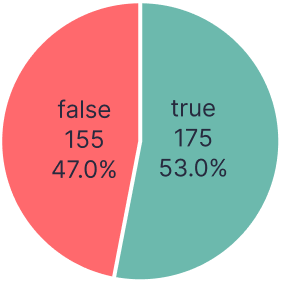
\includegraphics[width=\textwidth]{img/violations+passes.png}
	\caption{How many of all violations and tests combined are valid?}
	\label{fig:checks-validity-all}
	\end{subfigure}
\caption{Valididty of tests performed by addon-a11y}
\label{fig:checks-validity}
\end{figure}

\textbf{RQ2}: "What kind of errors can be caught by running automated accessibility tests on a component library?" can be answered based on these results and the results from manually evaluating the same components. The \ac{wcag} Success Criterion that proved to be reliably testable in Pipedrive's component library are:

\begin{itemize}
	\item Success Criterion 1.1.1 Non-text Content
	% (https://www.w3.org/TR/WCAG21/#non-text-content)
	% \begin{itemize}
	% 	\item Images must have alternate text
	% \end{itemize}

	\item Success Criterion 1.3.1 Info and Relationships
	% https://www.w3.org/TR/WCAG21/#info-and-relationships
	% \begin{itemize}
	% 	\item Certain ARIA roles must contain particular children
	% \end{itemize}

	\item Success Criterion 1.4.3 Contrast (Minimum)
	% (https://www.w3.org/TR/WCAG21/\#contrast-minimum)
	\item Success Criterion 1.4.6 Contrast (Enhanced)
	% (https://www.w3.org/TR/WCAG21/\#contrast-enhanced)
	% \begin{itemize}
	% 	\item Color contrast
	% \end{itemize}

	\item Success Criterion 1.4.12 Text Spacing
	% (https://www.w3.org/TR/WCAG21/#text-spacing)
	% \begin{itemize}
	% 	\item Inline text spacing must be adjustable with custom stylesheets
	% \end{itemize}

	\item Success Criterion 2.1.1 Keyboard
	\item Success Criterion 2.1.3 Keyboard (No Exception)
	% (https://www.w3.org/TR/WCAG21/#keyboard)
	% (https://www.w3.org/TR/WCAG21/#keyboard-no-exception)
	% \begin{itemize}
	% 	\item Scrollable region must have keyboard access
	% \end{itemize}

	\item Success Criterion 2.4.4 Link Purpose (In Context)
	\item Success Criterion 2.4.9 Link Purpose (Link Only)
	% (https://www.w3.org/TR/WCAG21/#link-purpose-in-context)
	% (https://www.w3.org/TR/WCAG21/#link-purpose-link-only)
	% \begin{itemize}
	% 	\item Links with the same name must have a similar purpose
	% 	\item Links must have discernible text
	% \end{itemize}

	\item Success Criterion 4.1.1 Parsing
	% (https://www.w3.org/TR/WCAG21/#parsing)
	% \begin{itemize}
	% 	\item IDs used in ARIA and labels must be unique
	% \end{itemize}

	\item Success Criterion 4.1.2 Name, Role, Value
	% (https://www.w3.org/TR/WCAG21/\#name-role-value)
	% \begin{itemize}
	% 	\item Buttons must have discernible text
	% 	\item Form elements must have labels
	% 	\item Form field must not have multiple label elements
	% 	\item Form elements should have a visible label
	% 	\item ARIA input fields must have an accessible name
	% 	\item ARIA roles used must conform to valid values
	% 	\item ARIA commands must have an accessible name
	% 	\item Interactive controls must not be nested
	% \end{itemize}

	% \item Correct usage of WAI-ARIA
	% (https://www.w3.org/TR/wai-aria-1.1/#usage)
	% \begin{itemize}
	% 	\item ARIA attributes must conform to valid values
	% 	\item ARIA attributes must conform to valid names
	% 	\item Elements must only use allowed ARIA attributes
	% 	\item Required ARIA attributes must be provided
	% \end{itemize}

	% \item Best Practices Rules
	% \begin{itemize}
	% 	\item ARIA role should be appropriate for the element
	% 	\item Elements should not have tab index greater than zero
	% 	\item Alternative text of images should not be repeated as text
	% 	\item Headings should not be empty
	% 	\item Heading levels should only increase by one
	% \end{itemize}
\end{itemize}

In addition to these axe-core automated accessibility testing engine tested for the correct usage of \ac{wai-aria} and best practices rules that are defined by the developers of the testing tool based on the accepted practices in the industry. There are other \ac{wcag} Success Criteria that the tool is also capable of testing, but that just was not represented by this certain set of components and examples.

The most common valid test result was color contrast with 45,1\% of all violations and passes being color contrast issues. It is also important to note that this tool can reliably test for the existence of the alt attribute in an image, but it is not capable of judging how accurate the meaning is or even if the image is purely decorative and should have an empty alt value.

Based on the additional issues found in the manual audit, it could be concluded that the following issues should be manually tested:
\begin{itemize}
	\item Focus states
	\item Navigating by using a keyboard
	\item Navigating and interacting by using a screen reader
	\item Recognizable color differences between semantically different variants of one component
	\item Images and what should be the value of their alt text
	\item Svgs and if they should have an aria-label
\end{itemize}

Evaluating the accessibility of focus states with automated testing could potentially be improved by using pseudo states add-on and writing better examples for components that would also display it in all relevant focus states.

% What could be improved in component examples to make them more testable
Inaccurate results and missed issues indicated problems with how the component examples have been written. The following things could be improved to get better results from automated testing:
\begin{itemize}
	\item Variants of components that are meant to be used on dark backgrounds should always be displayed on a dark background
	\item Examples where the component gets triggered by a button should be avoided when possible or made visible to the testing tool by other means
	\item Pseudo-classes (like hover, focus etc) of interactive elements should be displayed in examples
	\item Examples should be simple and display one component at a time to reduce the number of test being run that are irrelaant to the isolated component
\end{itemize}

\subsection{How Much Was Compliance with WCAG 2.1 Improved?}

\info{RQ3: To what extent can integrating automated testing into a component library's development pipeline help improve its compliance with \ac{wcag}?  }

One of the benefits of using automated testing tools is improved observability of the state of accessibility.
Multiple reports were generated in Pipedrive's component library during the time that the usage of the automated testing tool was observed. The report counts different issues and the for the purpose of this study and for observing the overall process that was made over time the whole number of detected violations were compared. (Figure \ref{fig:automted-reports}).

\begin{figure}[ht]
	\centering
	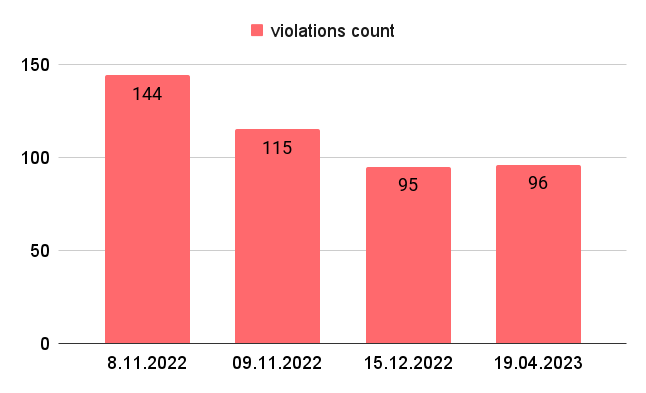
\includegraphics[width=0.8\textwidth]{img/automated-audit-reports.png}
	\caption{How much have automated audit report results improved since adding the tool?}
	\label{fig:automted-reports}
\end{figure}

Results over 5 months show that we reduced the highest number of accessibility issues while and just after conducting the manual accessibility audit. This is logical because the team involved in performing the audit also had dedicated time to focus on solving these issues. It is also worth noting that several new components have been added to the library during this time and the number of accessibility issues has not increased considerably.

As discussed in previous chapters automated accessibility can't catch all issues. So the fact that almost no additional violations have been added alone can't provide certainty that this component library is just as accessible as it was the last time the report was generated. It could be argued that the biggest value of using this in addition to finding certain kinds of accessibility violations has been bringing focus and attention to the subject of accessibility.

\citeauthor{Paterno2020} said that developers find maintaining a high level of accessibility hard because it is then only considered after the first release of the product. Having a continuous way to monitor and detect issues should help keep the level that was reached in the phase where there was more time to focus on accessibility. The data collected in the short time that this automated accessibility tool has been in use in Pipedrive supports that theory.

A good level of accessibility is easier to achieve when developers consider it from the start of the process. Fixing things, later on, is much harder to justify on the business side and might be more difficult than it would have been to build a component or a webpage keeping accessibility in mind from the beginning.

With the data collected during this research, it is not possible to say definitively that implementing automated accessibility testing in a component library's development workflow will improve the accessibility of the end product where these elements are being used, but there is data to support that it is very likely that it could improve it to some extent.

The experience of using these tools and conversations with other developers in the company has suggested that one big benefit of using tools like this is that it makes the whole subject of web accessibility a bit more measurable and less daunting. Having an easy familiar way of testing for accessibility violations together with links to resources that help in solving these issues will make it more likely for developers to take on the task of solving these issues.

\subsection{Limitations of Testing in Component Libraries}
\info{RQ4: What are the biggest problems of integrating automated accessibility testing into a component library's development workflow?}

\todo{Follow up survey + reach out to devs I know have used addon-a11y, button issue, not possible to add to CI currently - easy to not notice}
Considering that automated accessibility tests are not capable of evaluating all \ac{wcag} Success Criteria there are also additional limitations that apply when these tests are being run on isolated components. The context around the elements that are being used on a webpage is important to understand what the purpose of each element is. \ac{cdd} development methodology promotes first perfecting these isolated elements before moving on to the next step where they are combined to build up full views and logical interactions. This means that in component library testing it is not so important to focus on the things that depend on the final context, but rather on everything that is contained in the component. The assumption is that there should be additional testing in the next stages of development.

In the case study that was carried out in Pipedrive's component library, Storybook was used as a way of rendering the components and running automated tests on them. The accessibility add-on in Storybook analyzes the examples that have been made for the component and unsuitable examples can cause false results. Like components triggered by a button described before.

Another limitation of this tool currently is that the results can only be viewed inside Storybook. To see the number of passes and fails you need to open the accessibility tab for each component. In the case study an additional tool was used to generate a report that summarized all the violations, but generating the report needed some manual steps. It would be possible to automate this, but this would not be worth the effort, because the newest version of Storybook will provide better solutions. It will be possible to run all accessibility checks as a part of the component's unit tests making it possible to add them to the \ac{ci} workflow.

\end{document}